\documentclass[10pt]{article}\usepackage[]{graphicx}\usepackage[]{color}
%% maxwidth is the original width if it is less than linewidth
%% otherwise use linewidth (to make sure the graphics do not exceed the margin)
\makeatletter
\def\maxwidth{ %
  \ifdim\Gin@nat@width>\linewidth
    \linewidth
  \else
    \Gin@nat@width
  \fi
}
\makeatother

\definecolor{fgcolor}{rgb}{0.345, 0.345, 0.345}
\newcommand{\hlnum}[1]{\textcolor[rgb]{0.686,0.059,0.569}{#1}}%
\newcommand{\hlstr}[1]{\textcolor[rgb]{0.192,0.494,0.8}{#1}}%
\newcommand{\hlcom}[1]{\textcolor[rgb]{0.678,0.584,0.686}{\textit{#1}}}%
\newcommand{\hlopt}[1]{\textcolor[rgb]{0,0,0}{#1}}%
\newcommand{\hlstd}[1]{\textcolor[rgb]{0.345,0.345,0.345}{#1}}%
\newcommand{\hlkwa}[1]{\textcolor[rgb]{0.161,0.373,0.58}{\textbf{#1}}}%
\newcommand{\hlkwb}[1]{\textcolor[rgb]{0.69,0.353,0.396}{#1}}%
\newcommand{\hlkwc}[1]{\textcolor[rgb]{0.333,0.667,0.333}{#1}}%
\newcommand{\hlkwd}[1]{\textcolor[rgb]{0.737,0.353,0.396}{\textbf{#1}}}%
\let\hlipl\hlkwb

\usepackage{framed}
\makeatletter
\newenvironment{kframe}{%
 \def\at@end@of@kframe{}%
 \ifinner\ifhmode%
  \def\at@end@of@kframe{\end{minipage}}%
  \begin{minipage}{\columnwidth}%
 \fi\fi%
 \def\FrameCommand##1{\hskip\@totalleftmargin \hskip-\fboxsep
 \colorbox{shadecolor}{##1}\hskip-\fboxsep
     % There is no \\@totalrightmargin, so:
     \hskip-\linewidth \hskip-\@totalleftmargin \hskip\columnwidth}%
 \MakeFramed {\advance\hsize-\width
   \@totalleftmargin\z@ \linewidth\hsize
   \@setminipage}}%
 {\par\unskip\endMakeFramed%
 \at@end@of@kframe}
\makeatother

\definecolor{shadecolor}{rgb}{.97, .97, .97}
\definecolor{messagecolor}{rgb}{0, 0, 0}
\definecolor{warningcolor}{rgb}{1, 0, 1}
\definecolor{errorcolor}{rgb}{1, 0, 0}
\newenvironment{knitrout}{}{} % an empty environment to be redefined in TeX

\usepackage{alltt}

\usepackage{amsmath,amssymb,amsthm}
\usepackage{fancyhdr,url,hyperref}
\usepackage{graphicx,xspace}
\usepackage{tikz}
\usetikzlibrary{shapes,arrows,decorations.pathmorphing,backgrounds,positioning,fit,through}
\oddsidemargin 0in  %0.5in
\topmargin     0in
\leftmargin    0in
\rightmargin   0in
\textheight    9in
\textwidth     6in %6in
%\headheight    0in
%\headsep       0in
%\footskip      0.5in

\newtheorem{thm}{Theorem}
\newtheorem{cor}[thm]{Corollary}
\newtheorem{obs}{Observation}
\newtheorem{lemma}{Lemma}
\newtheorem{claim}{Claim}
\newtheorem{definition}{Definition}
\newtheorem{question}{Question}
\newtheorem{answer}{Answer}
\newtheorem{problem}{Problem}
\newtheorem{solution}{Solution}
\newtheorem{conjecture}{Conjecture}

\pagestyle{fancy}

\lhead{\textsc{Prof. McNamara}}
\chead{\textsc{STAT 320: Lecture notes}}
\lfoot{}
\cfoot{}
%\cfoot{\thepage}
\rfoot{}
\renewcommand{\headrulewidth}{0.2pt}
\renewcommand{\footrulewidth}{0.0pt}

\newcommand{\ans}{\vspace{0.25in}}
\newcommand{\R}{{\sf R}\xspace}
\newcommand{\cmd}[1]{\texttt{#1}}
\DeclareMathOperator{\Ex}{\mathbb{E}}
\DeclareMathOperator{\Var}{\text{Var}}
\DeclareMathOperator{\X}{\mathbf{X}}
\DeclareMathOperator{\Hatmat}{\mathbf{H}}

\rhead{\textsc{November 6, 2018}}
\IfFileExists{upquote.sty}{\usepackage{upquote}}{}
\begin{document}

\paragraph{Agenda}
\begin{enumerate}
  \itemsep0em
  \item two-way ANOVA
  \item Interaction plots
  \item two-way ANOVA with interaction
\end{enumerate}



\paragraph{Two-way ANOVA}

\begin{table}[htbp]
\begin{tabular}{l|lllll|l}
& Adam & Brenda & Cathy & Dave & Emily & Mean \\ \hline
Exam 1 & 62 & 94 & 68 & 86 & 50 & 72 \\
Exam 2 & 87 & 95 & 93 & 97 & 63 & 87 \\
Exam 3 & 74 & 86 & 83 & 70 & 28 & 68 \\
Exam 4 & 77 & 89 & 73 & 79 & 47 & 73 \\ \hline
Mean & 75 & 91 & 79 & 83 & 47 & 75 \\
\end{tabular}
\end{table}

Simple block design has two factors with exactly one data value (observation) in each combination of the factors

Factor A has K levels, Factor B has J levels, so $n = KJ$ values.

\begin{eqnarray*}
Y = \mu + \alpha_k + \beta_j + \epsilon
\end{eqnarray*}


To compute the ANOVA, find the mean for each treatment (row means), each block (column means) and grand mean. Partitition the SST into three pieces:

\begin{eqnarray*}
SST = SSA + SSB + SSE \\
SSE = \sum(y_i-\bar{y})^2 = (n-1)s_Y^2 \\
SSA = \sum J(\bar{y}_k-\bar{y})^2 \\
SSB = \sum K(\bar{y}_j-\bar{y})^2 \\
SSE = SST - SSA - SSB
\end{eqnarray*}

If you get the R output, it will look something like this

\begin{table}[htbp]
\begin{tabular}{l|l|l|l|l|l}
& df & SS & MS & F & p-value \\ \hline
Trts/A & K-1 & SSA & SSA/(K-1) & MS/MSE & \\ \hline
Block & J-1 & SSB & SSB/(J-1) & MSB/MSE & \\ \hline
Error & (K-1)(J-1) & SSE & SSE/(K-1)(J -1) & & \\ \hline
Total & n-1 & SST & & & 
\end{tabular}
\end{table}

This tests two hypotheses:

\begin{eqnarray*}
&H_0:& \alpha_1=\alpha_2=\dots=\alpha_k=0 \\
&H_A:& \text{at least one } \alpha_k\neq0 
\end{eqnarray*}

\begin{eqnarray*}
&H_0:& \beta_1=\beta_2=\dots=\beta_j=0 \\
&H_A:& \text{at least one } \beta_j\neq0 
\end{eqnarray*}


\paragraph{Interaction plots}

A common way to visualize the interaction between two categorical variables is with an interaction plot. 

\begin{figure}[htbp]
\begin{center}
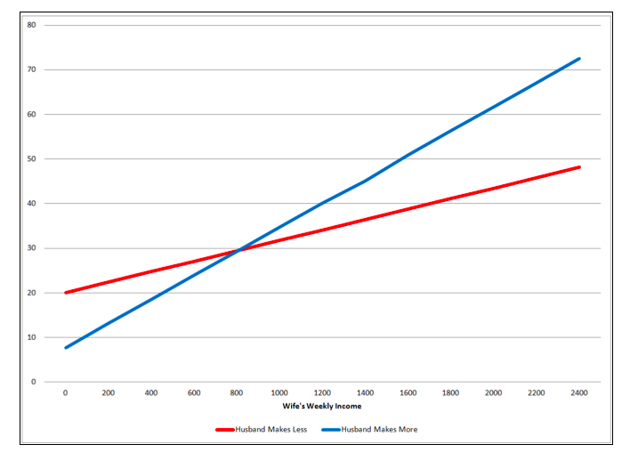
\includegraphics[width=0.7\textwidth]{Atlantic_Chores.png}
\caption{Figure from the Atlantic article, ``Emasculated Men Refuse to Do Chores--Except Cooking.'' \label{atlantic}}
\end{center}
\end{figure}

As an example, consider Figure \ref{atlantic}, from \url{https://www.theatlantic.com/health/archive/2016/10/the-only-chore-men-will-do-is-cook/505067/}

This is an example from regression (so the x-axis has meaning) but we also commonly see them for ANOVA. 

Example: glue strength

\begin{knitrout}
\definecolor{shadecolor}{rgb}{0.969, 0.969, 0.969}\color{fgcolor}\begin{kframe}
\begin{alltt}
\hlkwd{library}\hlstd{(tidyverse)}
\end{alltt}


{\ttfamily\noindent\itshape\color{messagecolor}{\#\# -- Attaching packages ------------------------------------------------------------------------ tidyverse 1.2.1 --}}

{\ttfamily\noindent\itshape\color{messagecolor}{\#\# v ggplot2 3.0.0\ \ \ \  v purrr\ \  0.2.5\\\#\# v tibble\ \ 1.4.2\ \ \ \  v dplyr\ \  0.7.7\\\#\# v tidyr\ \  0.8.1\ \ \ \  v stringr 1.3.1\\\#\# v readr\ \  1.1.1\ \ \ \  v forcats 0.3.0}}

{\ttfamily\noindent\itshape\color{messagecolor}{\#\# -- Conflicts --------------------------------------------------------------------------- tidyverse\_conflicts() --\\\#\# x dplyr::filter() masks stats::filter()\\\#\# x dplyr::lag()\ \ \ \ masks stats::lag()}}\begin{alltt}
\hlstd{GlueStrength} \hlkwb{<-} \hlkwd{data.frame}\hlstd{(}\hlkwc{Plastic} \hlstd{=} \hlkwd{c}\hlstd{(}\hlnum{52}\hlstd{,}\hlnum{64}\hlstd{,}\hlnum{67}\hlstd{,}\hlnum{55}\hlstd{,}\hlnum{86}\hlstd{,}\hlnum{72}\hlstd{),} \hlkwc{Wood} \hlstd{=} \hlkwd{c}\hlstd{(}\hlnum{72}\hlstd{,}\hlnum{60}\hlstd{,}\hlnum{78}\hlstd{,}\hlnum{68}\hlstd{,}\hlnum{43}\hlstd{,}\hlnum{51}\hlstd{),} \hlkwc{Thickness} \hlstd{=} \hlkwd{c}\hlstd{(}\hlkwd{rep}\hlstd{(}\hlstr{"Thin"}\hlstd{,} \hlkwc{times}\hlstd{=}\hlnum{2}\hlstd{),} \hlkwd{rep}\hlstd{(}\hlstr{"Moderate"}\hlstd{,} \hlkwc{times}\hlstd{=}\hlnum{2}\hlstd{),} \hlkwd{rep}\hlstd{(}\hlstr{"Heavy"}\hlstd{,} \hlkwc{times}\hlstd{=}\hlnum{2}\hlstd{)))}
\hlstd{GlueStrengthRS} \hlkwb{<-} \hlstd{GlueStrength} \hlopt \hlkwd{gather}\hlstd{(glue,force,}\hlopt{-}\hlstd{Thickness)}
\end{alltt}
\end{kframe}
\end{knitrout}


\begin{knitrout}
\definecolor{shadecolor}{rgb}{0.969, 0.969, 0.969}\color{fgcolor}\begin{kframe}
\begin{alltt}
\hlstd{GlueStrengthRS} \hlopt
  \hlkwd{group_by}\hlstd{(glue)} \hlopt
  \hlkwd{summarize}\hlstd{(}\hlkwd{mean}\hlstd{(force))}
\end{alltt}
\begin{verbatim}
## # A tibble: 2 x 2
##   glue    `mean(force)`
##   <chr>           <dbl>
## 1 Plastic            66
## 2 Wood               62
\end{verbatim}
\end{kframe}
\end{knitrout}


\begin{knitrout}
\definecolor{shadecolor}{rgb}{0.969, 0.969, 0.969}\color{fgcolor}\begin{kframe}
\begin{alltt}
\hlkwd{interaction.plot}\hlstd{(GlueStrengthRS}\hlopt{$}\hlstd{Thickness, GlueStrengthRS}\hlopt{$}\hlstd{glue, GlueStrengthRS}\hlopt{$}\hlstd{force)}
\end{alltt}
\end{kframe}
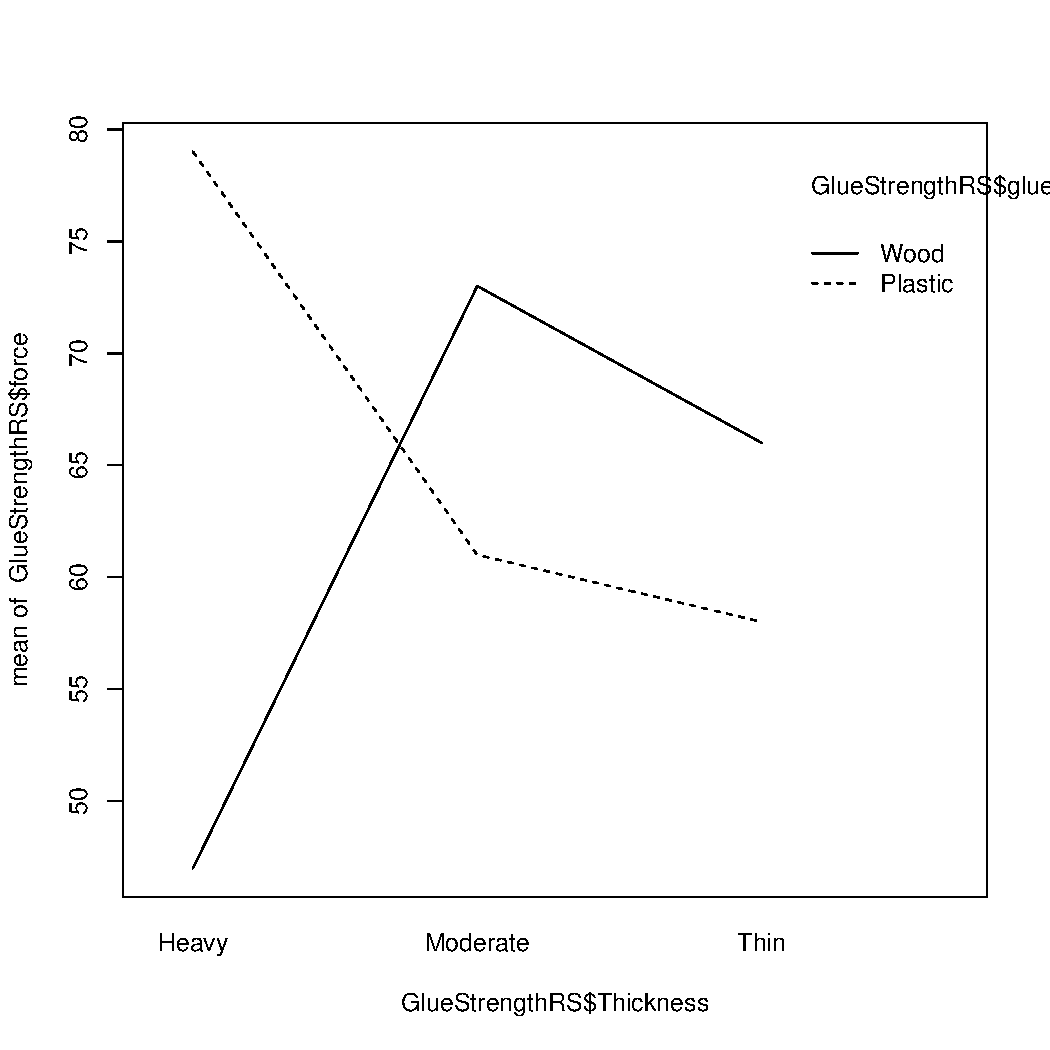
\includegraphics[width=\maxwidth]{figure/unnamed-chunk-3-1} 
\begin{kframe}\begin{alltt}
\hlkwd{interaction.plot}\hlstd{(GlueStrengthRS}\hlopt{$}\hlstd{glue, GlueStrengthRS}\hlopt{$}\hlstd{Thickness, GlueStrengthRS}\hlopt{$}\hlstd{force)}
\end{alltt}
\end{kframe}
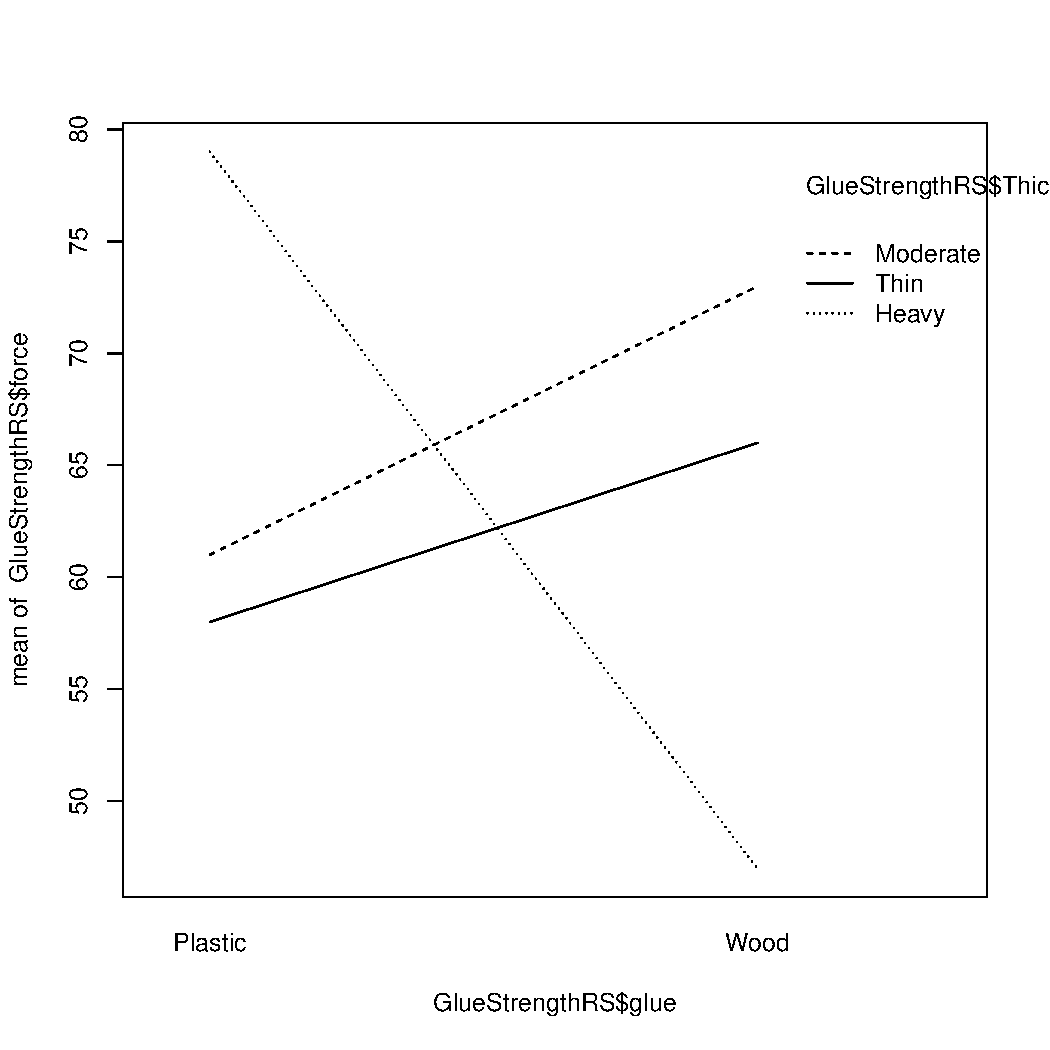
\includegraphics[width=\maxwidth]{figure/unnamed-chunk-3-2} 

\end{knitrout}

\begin{knitrout}
\definecolor{shadecolor}{rgb}{0.969, 0.969, 0.969}\color{fgcolor}\begin{kframe}
\begin{alltt}
\hlstd{a1} \hlkwb{<-} \hlkwd{aov}\hlstd{(force}\hlopt{~}\hlstd{Thickness}\hlopt{+}\hlstd{glue}\hlopt{+}\hlstd{Thickness}\hlopt{*}\hlstd{glue,} \hlkwc{data}\hlstd{=GlueStrengthRS)}
\hlkwd{summary}\hlstd{(a1)}
\end{alltt}
\begin{verbatim}
##                Df Sum Sq Mean Sq F value Pr(>F)  
## Thickness       2     56      28   0.424 0.6725  
## glue            1     48      48   0.727 0.4265  
## Thickness:glue  2   1184     592   8.970 0.0157 *
## Residuals       6    396      66                 
## ---
## Signif. codes:  0 '***' 0.001 '**' 0.01 '*' 0.05 '.' 0.1 ' ' 1
\end{verbatim}
\end{kframe}
\end{knitrout}


\begin{eqnarray*}
Y = \mu + \alpha_k + \beta_j + \gamma_{kj} + \epsilon
\end{eqnarray*}

\begin{eqnarray*}
SST = SSA + SSB + SSAB + SSE
\end{eqnarray*}


%Note to self: next time I should include more of the computation/comparison of anova() on a pair of linear models and aov() on a multi-term model. 
\end{document}
